% Options for packages loaded elsewhere
\PassOptionsToPackage{unicode}{hyperref}
\PassOptionsToPackage{hyphens}{url}
\PassOptionsToPackage{dvipsnames,svgnames,x11names}{xcolor}
%
\documentclass[
  letterpaper,
  DIV=11,
  numbers=noendperiod]{scrartcl}

\usepackage{amsmath,amssymb}
\usepackage{iftex}
\ifPDFTeX
  \usepackage[T1]{fontenc}
  \usepackage[utf8]{inputenc}
  \usepackage{textcomp} % provide euro and other symbols
\else % if luatex or xetex
  \usepackage{unicode-math}
  \defaultfontfeatures{Scale=MatchLowercase}
  \defaultfontfeatures[\rmfamily]{Ligatures=TeX,Scale=1}
\fi
\usepackage{lmodern}
\ifPDFTeX\else  
    % xetex/luatex font selection
\fi
% Use upquote if available, for straight quotes in verbatim environments
\IfFileExists{upquote.sty}{\usepackage{upquote}}{}
\IfFileExists{microtype.sty}{% use microtype if available
  \usepackage[]{microtype}
  \UseMicrotypeSet[protrusion]{basicmath} % disable protrusion for tt fonts
}{}
\makeatletter
\@ifundefined{KOMAClassName}{% if non-KOMA class
  \IfFileExists{parskip.sty}{%
    \usepackage{parskip}
  }{% else
    \setlength{\parindent}{0pt}
    \setlength{\parskip}{6pt plus 2pt minus 1pt}}
}{% if KOMA class
  \KOMAoptions{parskip=half}}
\makeatother
\usepackage{xcolor}
\usepackage[top=30mm,left=20mm]{geometry}
\setlength{\emergencystretch}{3em} % prevent overfull lines
\setcounter{secnumdepth}{5}
% Make \paragraph and \subparagraph free-standing
\ifx\paragraph\undefined\else
  \let\oldparagraph\paragraph
  \renewcommand{\paragraph}[1]{\oldparagraph{#1}\mbox{}}
\fi
\ifx\subparagraph\undefined\else
  \let\oldsubparagraph\subparagraph
  \renewcommand{\subparagraph}[1]{\oldsubparagraph{#1}\mbox{}}
\fi

\usepackage{color}
\usepackage{fancyvrb}
\newcommand{\VerbBar}{|}
\newcommand{\VERB}{\Verb[commandchars=\\\{\}]}
\DefineVerbatimEnvironment{Highlighting}{Verbatim}{commandchars=\\\{\}}
% Add ',fontsize=\small' for more characters per line
\usepackage{framed}
\definecolor{shadecolor}{RGB}{241,243,245}
\newenvironment{Shaded}{\begin{snugshade}}{\end{snugshade}}
\newcommand{\AlertTok}[1]{\textcolor[rgb]{0.68,0.00,0.00}{#1}}
\newcommand{\AnnotationTok}[1]{\textcolor[rgb]{0.37,0.37,0.37}{#1}}
\newcommand{\AttributeTok}[1]{\textcolor[rgb]{0.40,0.45,0.13}{#1}}
\newcommand{\BaseNTok}[1]{\textcolor[rgb]{0.68,0.00,0.00}{#1}}
\newcommand{\BuiltInTok}[1]{\textcolor[rgb]{0.00,0.23,0.31}{#1}}
\newcommand{\CharTok}[1]{\textcolor[rgb]{0.13,0.47,0.30}{#1}}
\newcommand{\CommentTok}[1]{\textcolor[rgb]{0.37,0.37,0.37}{#1}}
\newcommand{\CommentVarTok}[1]{\textcolor[rgb]{0.37,0.37,0.37}{\textit{#1}}}
\newcommand{\ConstantTok}[1]{\textcolor[rgb]{0.56,0.35,0.01}{#1}}
\newcommand{\ControlFlowTok}[1]{\textcolor[rgb]{0.00,0.23,0.31}{#1}}
\newcommand{\DataTypeTok}[1]{\textcolor[rgb]{0.68,0.00,0.00}{#1}}
\newcommand{\DecValTok}[1]{\textcolor[rgb]{0.68,0.00,0.00}{#1}}
\newcommand{\DocumentationTok}[1]{\textcolor[rgb]{0.37,0.37,0.37}{\textit{#1}}}
\newcommand{\ErrorTok}[1]{\textcolor[rgb]{0.68,0.00,0.00}{#1}}
\newcommand{\ExtensionTok}[1]{\textcolor[rgb]{0.00,0.23,0.31}{#1}}
\newcommand{\FloatTok}[1]{\textcolor[rgb]{0.68,0.00,0.00}{#1}}
\newcommand{\FunctionTok}[1]{\textcolor[rgb]{0.28,0.35,0.67}{#1}}
\newcommand{\ImportTok}[1]{\textcolor[rgb]{0.00,0.46,0.62}{#1}}
\newcommand{\InformationTok}[1]{\textcolor[rgb]{0.37,0.37,0.37}{#1}}
\newcommand{\KeywordTok}[1]{\textcolor[rgb]{0.00,0.23,0.31}{#1}}
\newcommand{\NormalTok}[1]{\textcolor[rgb]{0.00,0.23,0.31}{#1}}
\newcommand{\OperatorTok}[1]{\textcolor[rgb]{0.37,0.37,0.37}{#1}}
\newcommand{\OtherTok}[1]{\textcolor[rgb]{0.00,0.23,0.31}{#1}}
\newcommand{\PreprocessorTok}[1]{\textcolor[rgb]{0.68,0.00,0.00}{#1}}
\newcommand{\RegionMarkerTok}[1]{\textcolor[rgb]{0.00,0.23,0.31}{#1}}
\newcommand{\SpecialCharTok}[1]{\textcolor[rgb]{0.37,0.37,0.37}{#1}}
\newcommand{\SpecialStringTok}[1]{\textcolor[rgb]{0.13,0.47,0.30}{#1}}
\newcommand{\StringTok}[1]{\textcolor[rgb]{0.13,0.47,0.30}{#1}}
\newcommand{\VariableTok}[1]{\textcolor[rgb]{0.07,0.07,0.07}{#1}}
\newcommand{\VerbatimStringTok}[1]{\textcolor[rgb]{0.13,0.47,0.30}{#1}}
\newcommand{\WarningTok}[1]{\textcolor[rgb]{0.37,0.37,0.37}{\textit{#1}}}

\providecommand{\tightlist}{%
  \setlength{\itemsep}{0pt}\setlength{\parskip}{0pt}}\usepackage{longtable,booktabs,array}
\usepackage{calc} % for calculating minipage widths
% Correct order of tables after \paragraph or \subparagraph
\usepackage{etoolbox}
\makeatletter
\patchcmd\longtable{\par}{\if@noskipsec\mbox{}\fi\par}{}{}
\makeatother
% Allow footnotes in longtable head/foot
\IfFileExists{footnotehyper.sty}{\usepackage{footnotehyper}}{\usepackage{footnote}}
\makesavenoteenv{longtable}
\usepackage{graphicx}
\makeatletter
\def\maxwidth{\ifdim\Gin@nat@width>\linewidth\linewidth\else\Gin@nat@width\fi}
\def\maxheight{\ifdim\Gin@nat@height>\textheight\textheight\else\Gin@nat@height\fi}
\makeatother
% Scale images if necessary, so that they will not overflow the page
% margins by default, and it is still possible to overwrite the defaults
% using explicit options in \includegraphics[width, height, ...]{}
\setkeys{Gin}{width=\maxwidth,height=\maxheight,keepaspectratio}
% Set default figure placement to htbp
\makeatletter
\def\fps@figure{htbp}
\makeatother

\KOMAoption{captions}{tableheading}
\makeatletter
\@ifpackageloaded{caption}{}{\usepackage{caption}}
\AtBeginDocument{%
\ifdefined\contentsname
  \renewcommand*\contentsname{Tabla de contenidos}
\else
  \newcommand\contentsname{Tabla de contenidos}
\fi
\ifdefined\listfigurename
  \renewcommand*\listfigurename{Listado de Figuras}
\else
  \newcommand\listfigurename{Listado de Figuras}
\fi
\ifdefined\listtablename
  \renewcommand*\listtablename{Listado de Tablas}
\else
  \newcommand\listtablename{Listado de Tablas}
\fi
\ifdefined\figurename
  \renewcommand*\figurename{Figura}
\else
  \newcommand\figurename{Figura}
\fi
\ifdefined\tablename
  \renewcommand*\tablename{Tabla}
\else
  \newcommand\tablename{Tabla}
\fi
}
\@ifpackageloaded{float}{}{\usepackage{float}}
\floatstyle{ruled}
\@ifundefined{c@chapter}{\newfloat{codelisting}{h}{lop}}{\newfloat{codelisting}{h}{lop}[chapter]}
\floatname{codelisting}{Listado}
\newcommand*\listoflistings{\listof{codelisting}{Listado de Listados}}
\makeatother
\makeatletter
\makeatother
\makeatletter
\@ifpackageloaded{caption}{}{\usepackage{caption}}
\@ifpackageloaded{subcaption}{}{\usepackage{subcaption}}
\makeatother
\ifLuaTeX
\usepackage[bidi=basic]{babel}
\else
\usepackage[bidi=default]{babel}
\fi
\babelprovide[main,import]{spanish}
% get rid of language-specific shorthands (see #6817):
\let\LanguageShortHands\languageshorthands
\def\languageshorthands#1{}
\ifLuaTeX
  \usepackage{selnolig}  % disable illegal ligatures
\fi
\usepackage{bookmark}

\IfFileExists{xurl.sty}{\usepackage{xurl}}{} % add URL line breaks if available
\urlstyle{same} % disable monospaced font for URLs
\hypersetup{
  pdftitle={Recomendación de anuncios},
  pdfauthor={Jorge Almonacid, Rubén Genillo, Humberto Pérez de la Blanca, Cristina Suárez; Universidad San Pablo CEU},
  pdflang={es},
  colorlinks=true,
  linkcolor={blue},
  filecolor={Maroon},
  citecolor={Blue},
  urlcolor={Blue},
  pdfcreator={LaTeX via pandoc}}

\title{Recomendación de anuncios}
\author{Jorge Almonacid, Rubén Genillo, Humberto Pérez de la Blanca,
Cristina Suárez \and Universidad San Pablo CEU}
\date{}

\begin{document}
\maketitle

\renewcommand*\contentsname{Indice}
{
\hypersetup{linkcolor=}
\setcounter{tocdepth}{3}
\tableofcontents
}
\textbf{ABSTRACT}

El proyecto se enfoca en la extracción y análisis de datos de Twitter
para la recomendación de anuncios personalizados. Para superar las
limitaciones de la API de Twitter, se implementaron técnicas de web
scraping con Twint y extracción de datos por ``fuerza bruta''. Con esta
información obtenida, se procedió a aplicar técnicas de análisis de
sentimientos para comprender las emociones expresadas en los
comentarios. Además, se utilizó el modelado de temas para identificar
los principales temas discutidos en la plataforma. Integrando estos
resultados, se desarrolló un sistema de asignación de anuncios dinámico
que se adapta a los temas identificados, mejorando así la relevancia y
efectividad de la publicidad dirigida.

\textbf{Palabras clave:} marketing - anuncios - sentiment analysis -
topic modeling

\newpage{}

\subsection{Introducción}\label{introducciuxf3n}

En el contexto del creciente panorama digital, la extracción y análisis
de datos de redes sociales se ha convertido en un componente crucial
para las estrategias de marketing y toma de decisiones empresariales. En
este proyecto, nos enfocamos en la aplicación de técnicas de
inteligencia artificial para la extracción, análisis y asignación de
anuncios basados en datos obtenidos de la plataforma Twitter.

\subsection{Brainstorming}\label{brainstorming}

Durante el brainstorming, se exploraron diversas áreas de interés, desde
la seguridad informática con el análisis de correos maliciosos y el
desarrollo de un detector de malware, hasta la aplicación de la teoría
de juegos para identificar posibles trampas, lo que representa un
enfoque innovador con amplias implicaciones. Además, se abordó el campo
de la inteligencia artificial con la creación de un modelo de generación
de texto, lo que refleja un interés en tecnologías avanzadas y su
impacto potencial.

Se seleccionó una idea centrada en el ámbito del análisis de datos en
redes sociales para la recomendación de anuncios. Esta propuesta
demuestra una comprensión perspicaz del papel cada vez más relevante que
desempeñan las opiniones y tendencias en línea en el mundo del marketing
digital.

\paragraph{Necesidades:}\label{necesidades}

Al haber seleccionado la idea centrada en el análisis de datos en redes
sociales para la recomendación de anuncios, se pone de manifiesto la
importancia de estar actualizados, ser precisos y comprender las
respuestas de los clientes. Estas necesidades reflejan la relevancia de
mantenerse al tanto de las tendencias cambiantes en línea, la precisión
en la interpretación de datos y la comprensión profunda de las
interacciones de los clientes en entornos digitales. Este enfoque
resalta la importancia estratégica del marketing en un mundo cada vez
más impulsado por la información y las interacciones en línea.

\subsection{Objetivo}\label{objetivo}

El objetivo de la extracción de datos y opiniones en redes sociales de
usuarios para la recomendación de anuncios se fundamenta en la necesidad
de acceder a información pública, en tiempo real y constantemente
actualizada. Este enfoque estratégico busca aprovechar la riqueza de
datos disponibles en entornos digitales públicos, garantizar la
relevancia y actualidad de la información recopilada, y capturar las
tendencias y opiniones más recientes. Al hacerlo, se busca informar
decisiones de marketing con datos dinámicos y significativos, alineados
con las demandas cambiantes del mercado y las interacciones de los
usuarios en línea.

Además, este enfoque puede tener usos alternativos significativos que
van más allá de la recomendación de anuncios. Por ejemplo, la extracción
de datos y opiniones en redes sociales puede ser invaluable para la
investigación de clientes, permitiendo una comprensión más profunda de
sus necesidades, preferencias y comportamientos en línea. Asimismo, la
identificación de \emph{Brand Ambassadors}, es decir, usuarios
influyentes que puedan promover de manera auténtica una marca, es otro
beneficio clave de esta estrategia. Además, el manejo de reputación en
línea se ve reforzado por la capacidad de monitorear y responder de
manera proactiva a las interacciones en redes sociales, lo que puede
impactar positivamente la percepción pública de una empresa o producto.
Estos son solo algunos ejemplos de cómo este enfoque puede ser
aprovechado para una variedad de aplicaciones estratégicas más allá de
la publicidad y recomendaciones comerciales.

\subsection{Tareas}\label{tareas}

La tarea se puede dividir en los siguientes temas:

\paragraph{Extracción de Datos:}\label{extracciuxf3n-de-datos}

En esta fase, se enfocará en la extracción de datos clave de la
plataforma Twitter. Se buscará obtener información pública de los
usuarios, como nombres, biografías, publicaciones, día y hora de
publicación, comentarios, interacciones como me gusta, seguidores,
seguidos y hashtags utilizados. Esta información será recopilada a
través de una API que permitirá acceder a estos datos de manera
estructurada. Además, se profundizará en la obtención de información
personal más detallada, como edad, género, localización, ocupación e
intereses de los usuarios para enriquecer el análisis.

\paragraph{Filtrar posts relevantes:}\label{filtrar-posts-relevantes}

Una vez recopilados los datos, el siguiente paso será filtrar y
clasificar los posts relevantes. Para lograr esto, se implementará un
análisis de temas avanzado. Se utilizarán algoritmos especializados como
el Análisis Semántico Latente (LSA) y la Asignación Latente de Dirichlet
(LDA) para identificar patrones y agrupar los posts según los temas
principales que abordan. Este proceso permitirá segmentar la información
de manera efectiva y comprender mejor las discusiones que tienen lugar
en la plataforma.

\paragraph{Análisis de sentimiento:}\label{anuxe1lisis-de-sentimiento}

Otro aspecto fundamental de esta tarea es el análisis de sentimiento.
Aquí se enfocará en determinar la polaridad de las opiniones expresadas
en los posts recopilados. Para ello, se emplearán lexicons de
sentimiento que ayudarán a clasificar las opiniones como positivas,
negativas o neutras. Además, se explorará un método alternativo que
involucra el uso de LMQL o langchain con Large Language Models para
mejorar la precisión y profundidad del análisis de sentimiento.

Se estudiarán detenidamente los datos obtenidos de Twitter para llevar a
cabo estas tareas con rigor y obtener información significativa que
puedan impulsar estrategias efectivas en marketing digital y toma de
decisiones empresariales.

\paragraph{Topic modeling:}\label{topic-modeling}

Finalmente aplicamos el topic modeling para categorizar automáticamente
los temas principales de los datos extraídos previamente, los cuales se
guardarán en una base de datos. Una vez tenemos los temas, se procederá
a la asignación de anuncios, los cuales serán clasificados mediante un
resumen por el mismo algoritmo de topic modeling y serán asignados a la
gente con las que coincidan los temas.

\newpage{}

\subsection{Diagramas}\label{diagramas}

Tuvimos que realizar 2 diagramas, por un lado el diagrama de desarrollo,
que muestra que actividades se van a realizar en el proyecto. Y por otro
lado el diagrama de Gantt, que se encarga de distribuir las tareas y
actividades en una línea temporal.

\begin{figure}[H]

{\centering 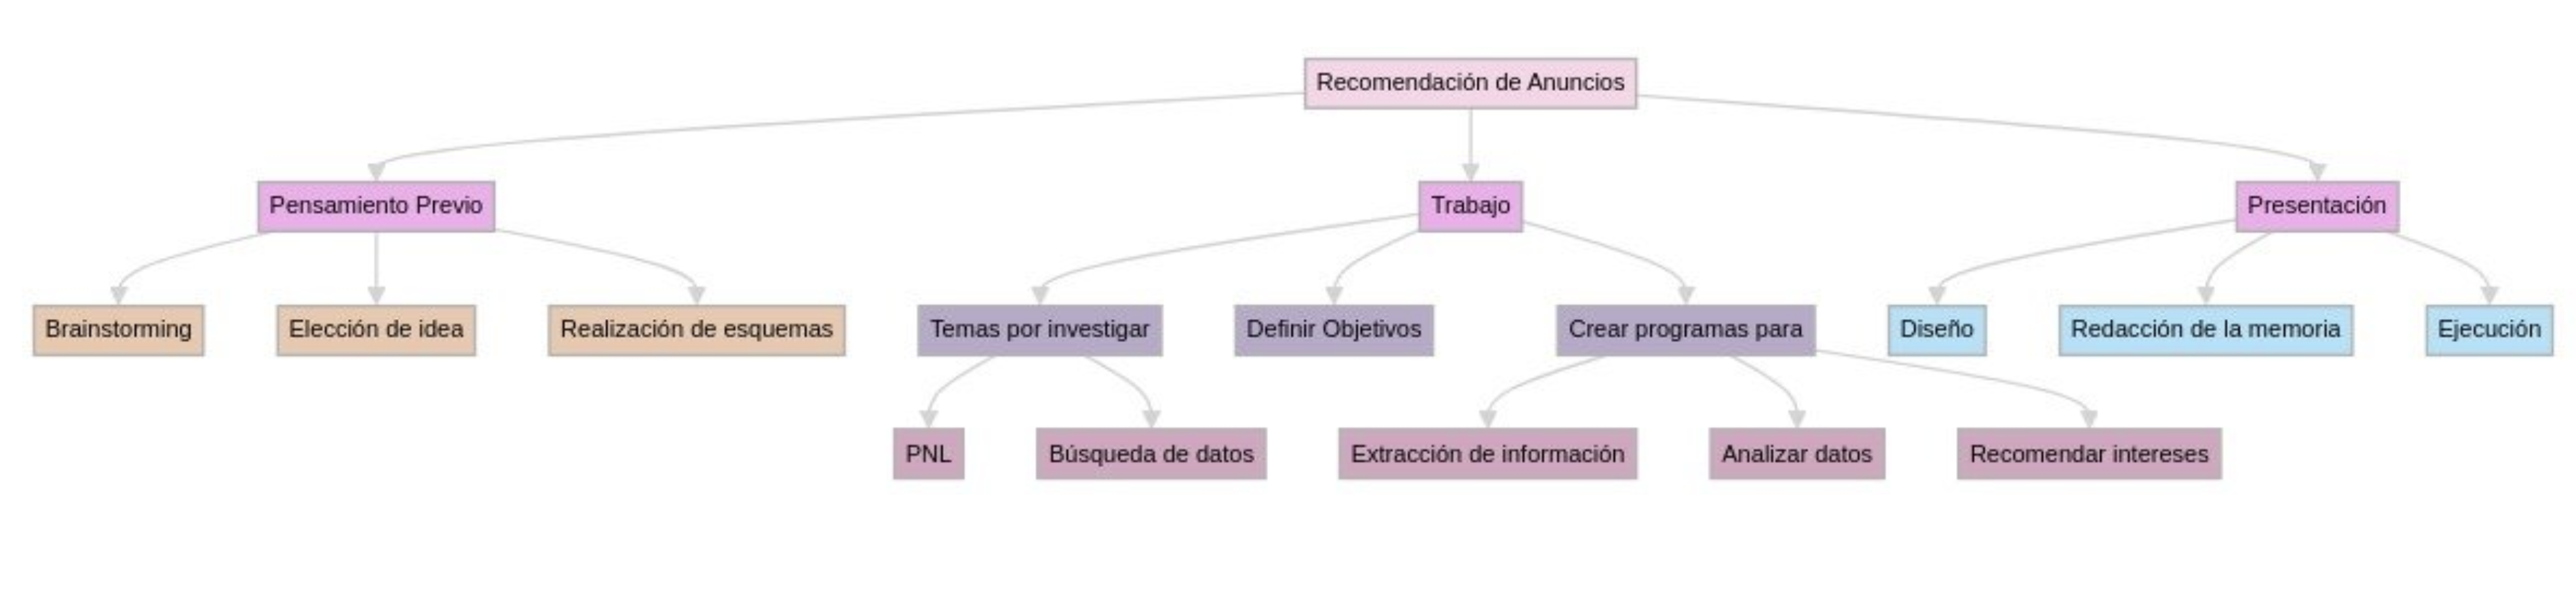
\includegraphics{diagrama de desarrollo.png}

}

\caption{Diagrama de desarrollo}

\end{figure}%

\begin{figure}[htbp]
    \centering
    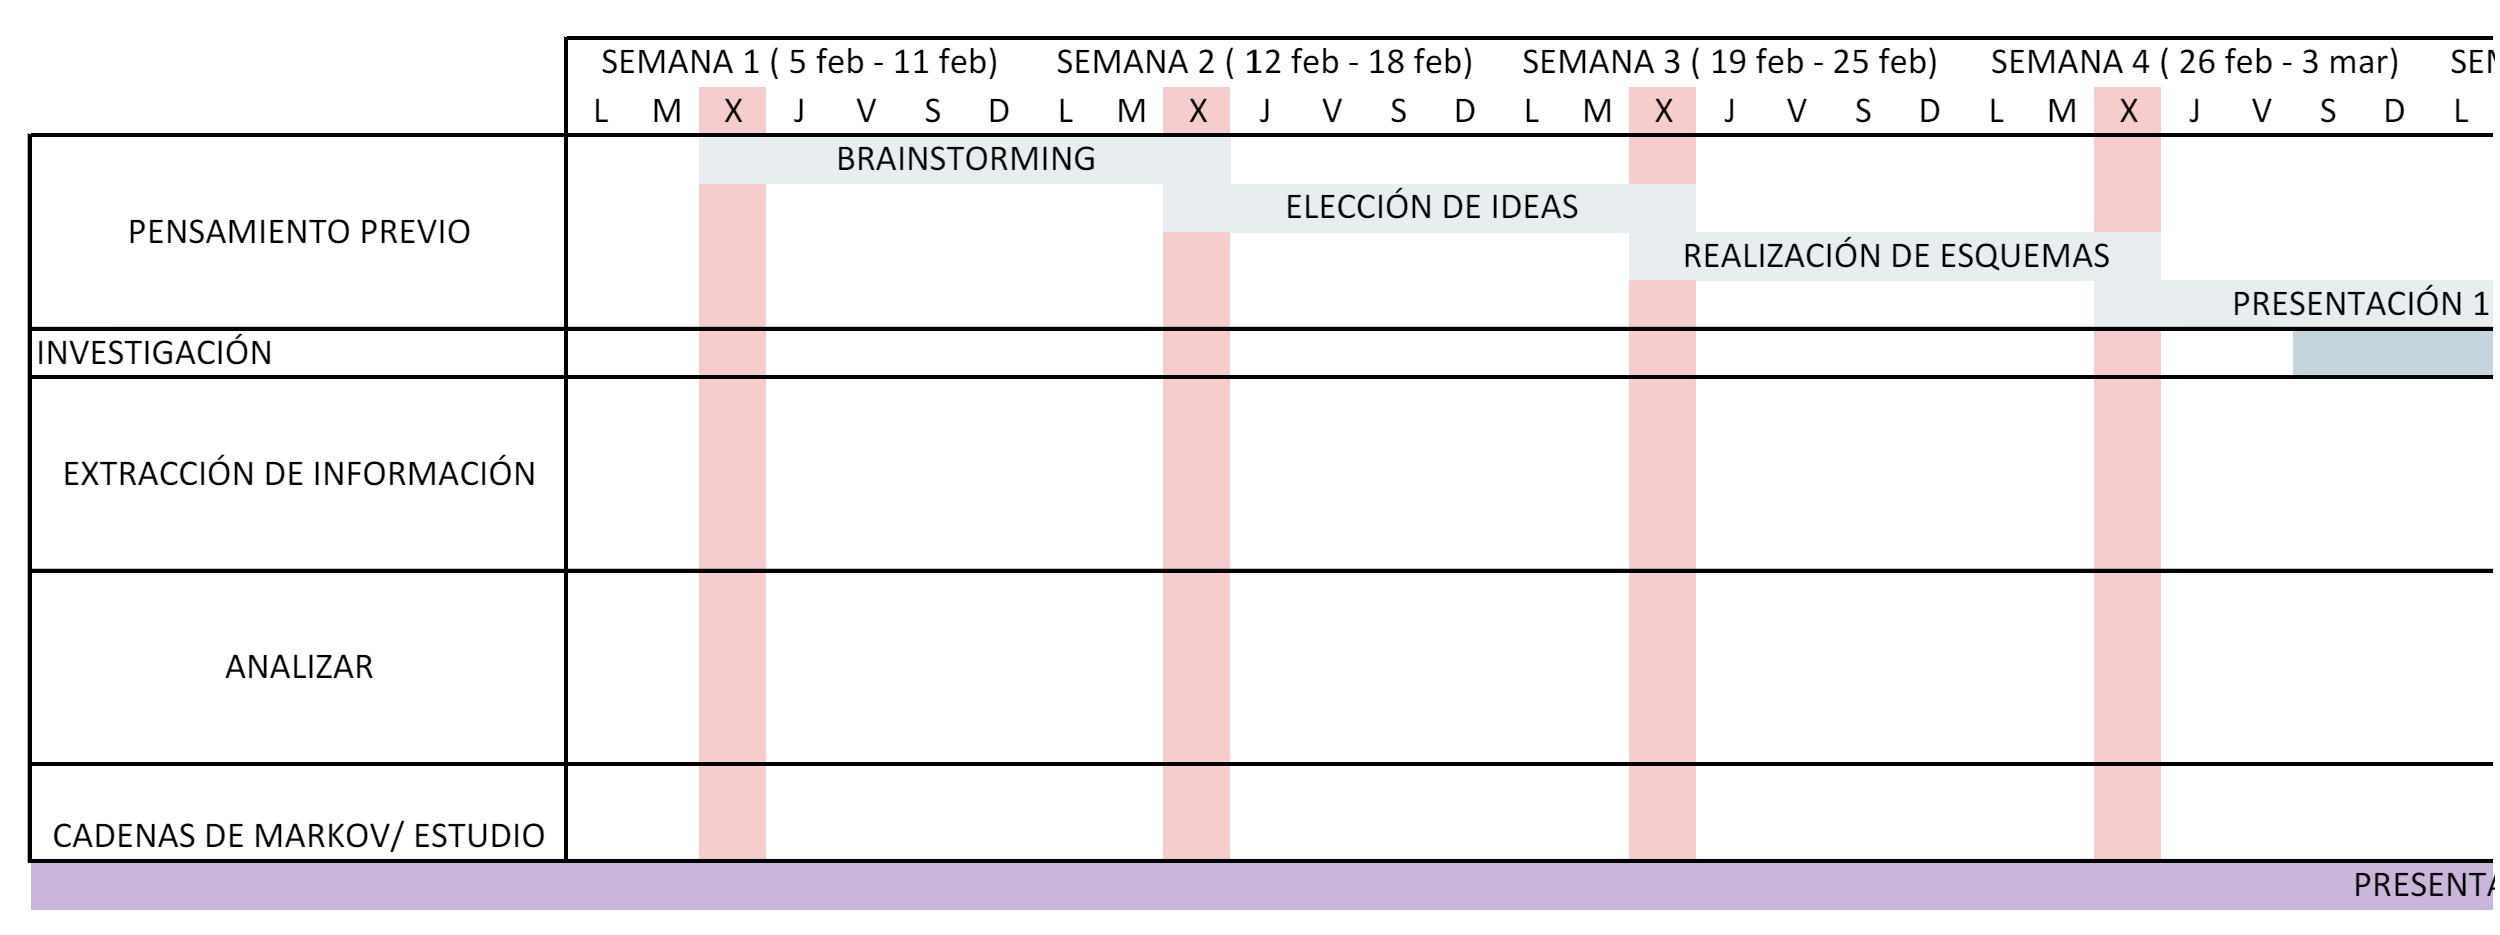
\includegraphics[width=0.8\textwidth, height=0.4\textheight]{gant1.png}
    \caption{Gant parte 1}
    \label{fig:gant1}
\end{figure}

\begin{figure}[htbp]
    \centering
    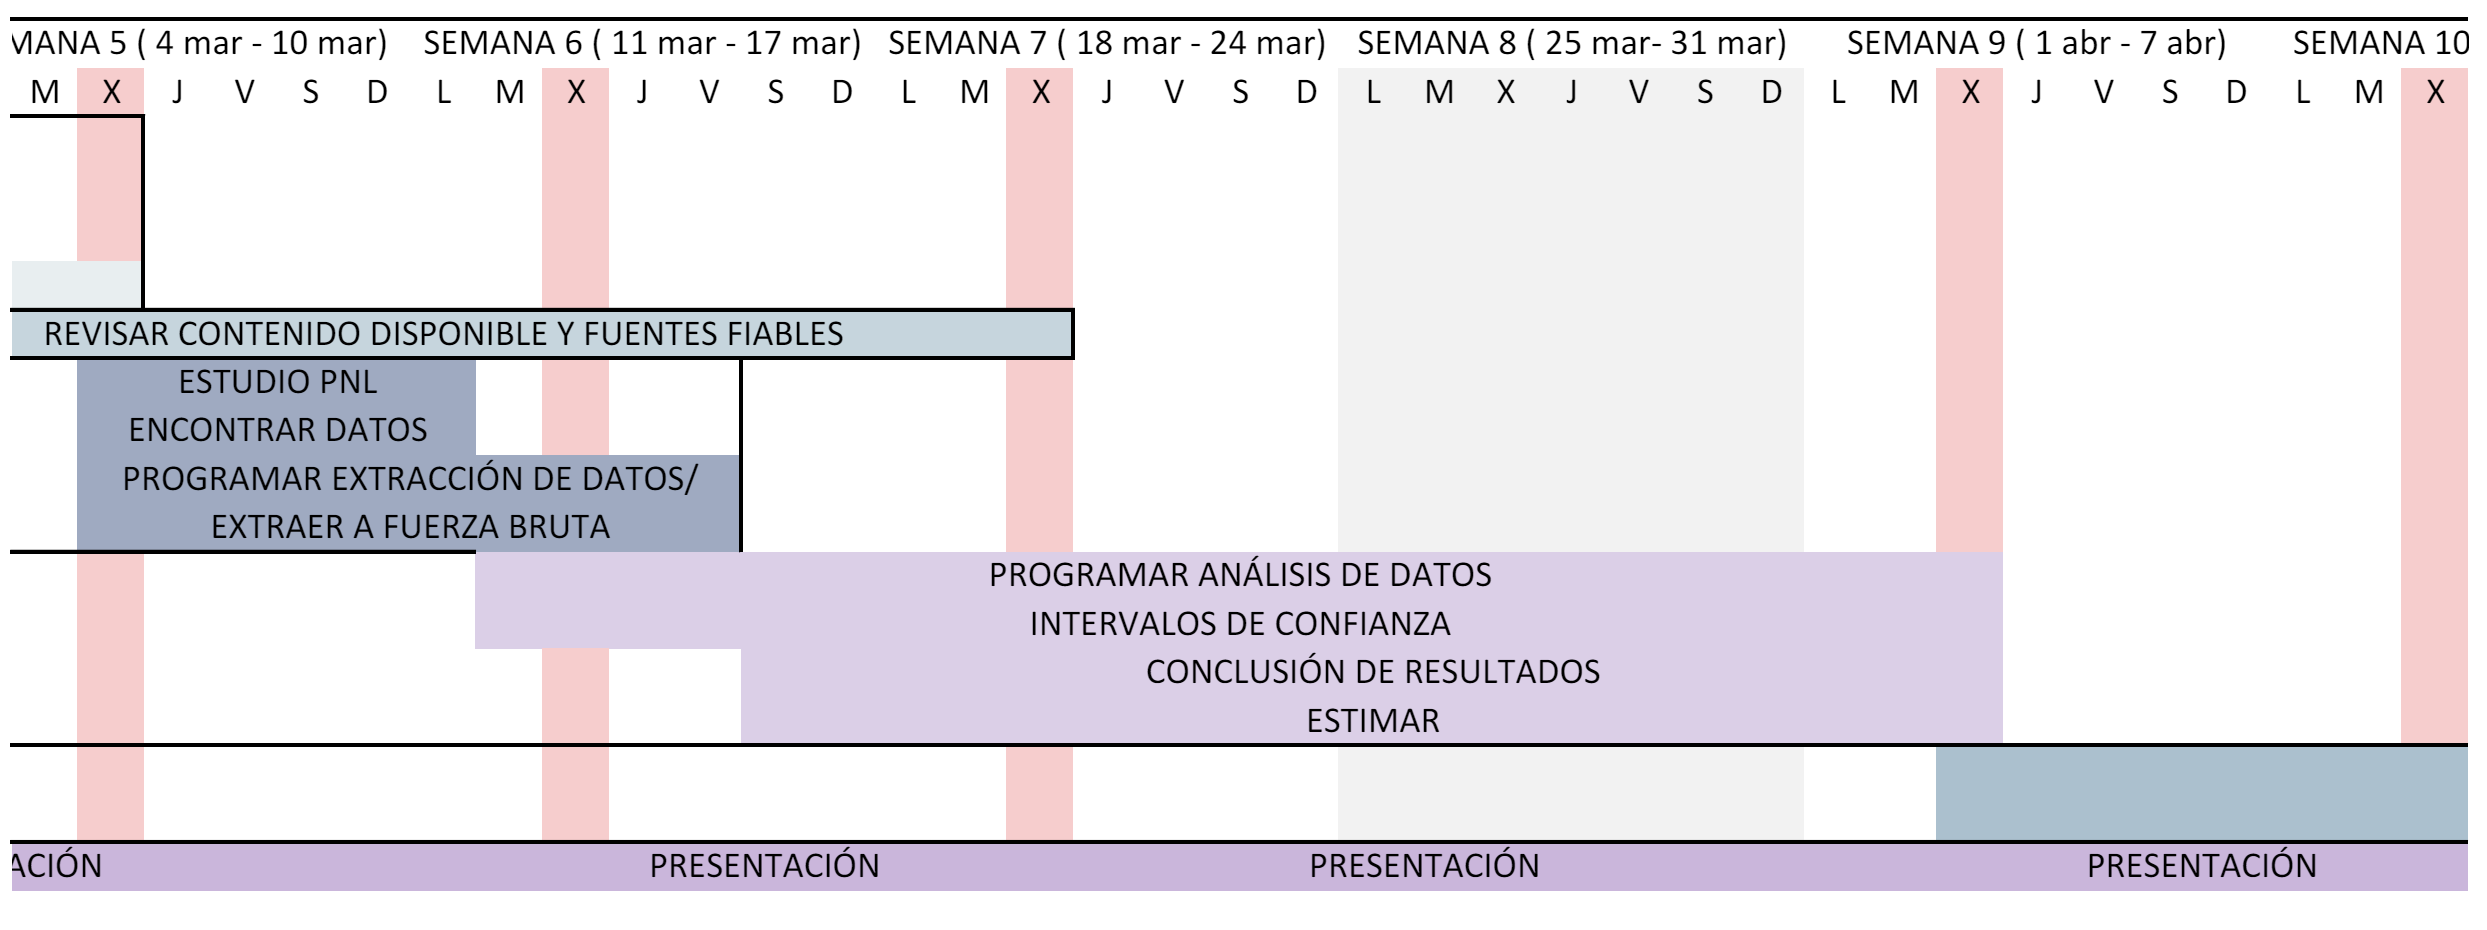
\includegraphics[width=0.8\textwidth, height=0.4\textheight]{gant2.png}
    \caption{Gant parte 2}
    \label{fig:gant2}
\end{figure}

\begin{figure}[htbp]
    \centering
    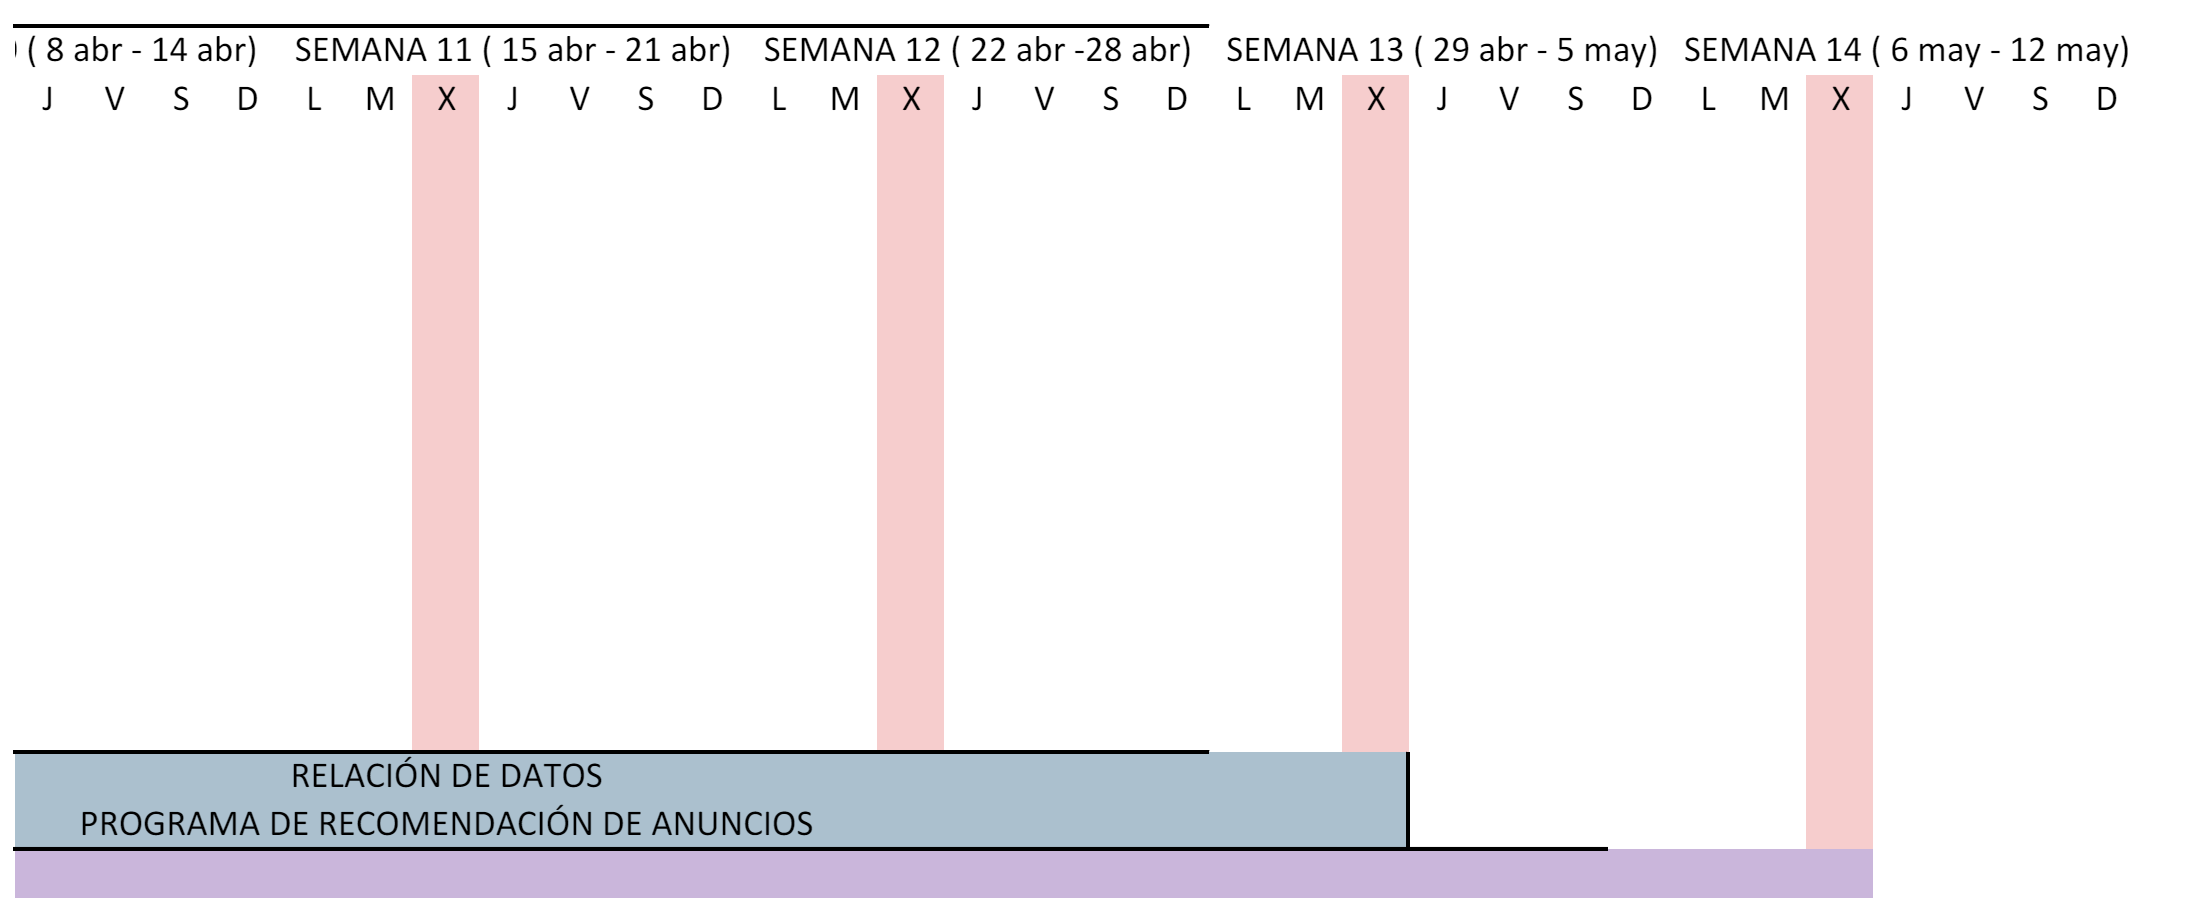
\includegraphics[width=0.8\textwidth, height=0.4\textheight]{gant3.png}
    \caption{Gantt parte 3}
    \label{fig:gantt3}
\end{figure}

\newpage{}

\subsection{Proyecto}\label{proyecto}

\paragraph{Extracción de datos}\label{extracciuxf3n-de-datos-1}

Durante la fase inicial de nuestro proyecto, nos encontramos con un
desafío inesperado al intentar extraer datos de la plataforma Twitter
utilizando su API, ya que las configuraciones de privacidad habían
experimentado cambios significativos, lo que nos impedía acceder a la
información de manera directa como habíamos planeado inicialmente. Ante
esta situación, optamos por un enfoque alternativo y eficaz mediante el
uso de Twint para realizar web scraping. Twint es una herramienta de
scraping para Twitter que nos permitió acceder a datos públicos
disponibles en perfiles y publicaciones, superando así las restricciones
impuestas por la API. Esta estrategia nos permitió recopilar una gran
cantidad de datos relevantes de manera eficiente y sin violar las
políticas de privacidad de la plataforma. Además, en paralelo a la
extracción de datos con Twint, estábamos utilizando una estrategia de
``fuerza bruta'' para recopilar información adicional. Esta técnica nos
permitió explorar exhaustivamente diversas fuentes de datos públicos,
complementando así los datos obtenidos a través del web scraping con
Twint. En resumen, el uso combinado de Twint y la extracción de datos
con fuerza bruta nos proporcionó una solución integral para obtener
datos valiosos de Twitter, sentando así las bases para nuestro posterior
análisis y recomendaciones.

\paragraph{IA para análisis de
sentimiento}\label{ia-para-anuxe1lisis-de-sentimiento}

El análisis de sentimiento implica la aplicación de técnicas avanzadas
de inteligencia artificial para comprender la carga emocional de los
mensajes expresados en las redes sociales.

El objetivo es determinar la polaridad de las opiniones y emociones de
los textos, en nuestro caso empleamos \emph{sentiment lexicons} basados
en unigramas. Estos nos proporcionan las emociones y sentimientos
asociados a las palabras individuales de un texto, tomando la emoción y
sentimiento de un texto como el mayor sentimiento en este.

El uso de sentiment lexicons frente a otras técnicas de sentiment
analysis ofrece la principal ventaja de ser más rápido, lo que es
necesario para hacer el cálculo rápido de opinión de muchos individuos.
Cabe aclarar que lo que conseguimos mediante los sentiments lexicons
realmente son la positvidad/neutralidad/negatividad de un texto, lo cual
no siempre significa siempre sacar una opinión final, ya que si el texto
habla muy negativamente sobre un tema y finalmente da un veredicto
positivo se puede ver muy influenciado por una mayor cantidad de
comentarios negativos y obtener que dicho texto habla negativamente. O
como, por ejemplo, citar el comentario negativo de otra persona en un
texto puede alterar negativamente el resultado positivo de un texto.

Iniciando nuestro análisis de sentimiento probamos distintos sentiment
lexicons con opiniones polares, ya que existen otros como
\emph{ncr}\footnote{El NRC Emotion Lexicon es una lista de palabras en inglés y sus asociaciones con ocho emociones básicas (ira, miedo, anticipación, confianza, sorpresa, tristeza, alegría y disgusto) y dos sentimientos (negativo y positivo).}
que son más concretos con el tipo de emoción, que fueron AFINN y bing.

\begin{itemize}
\item
  AFINN asigna a ciertas palabras una puntuación de entre -5 y 5, siendo
  una puntuación negativa un sentimiento negativo y una puntuación
  positiva un sentimiento positivo.
\item
  Bing directamente asigna el valor positivo o negativo a cada palabra.
\end{itemize}

A la hora de realizar test con texto extraído de twitter y comparar la
positividad del texto en si surgían varios inconvenientes. El primero
era que, por ejemplo, al analizar las opiniones en twitter del tráiler
de la última película de Deadpool se penalizaban palabras como
``Strange'', del nombre de un personaje de Marvel
\underline{Dr.Strange}, o ``KILLED'', que se refiera a la expresión
``they KILLED IT!!!'' siendo esta positiva, lo cual se puede llegar a
corregir (o incluso prever) al analizar las palabras con una emoción
asignada que más aparecen e ignorarlas. Otro problema que surge es no
capturar matices de su dominio como tomar en cuenta calificativos
delante de una palabra como ``no es bueno'' o ``no es cierto'',
sarcasmo, o en general ideas que dependan del contexto. Dados los
problemas surge una alternativa, VADER.

VADER \emph{(Valence Aware Dictionary and sEntiment Reasoner)} es un
sentiment lexicon basado en reglas gramaticales diseñado específicamente
para analizar sentimientos expresados en redes sociales. VADER es capaz
de analizar la positidad/neutralidad/negatividad un texto y dar un
puntuaje ente -1 y 1, y al estar basado en reglas gramaticales soluciona
la mayoría de los principales problemas como la negación o el uso de
exclamaciones, e incluso tomar la intensidad de palabras en mayúsculas o
tomar sentimientos de emojis hechos con caracteres como `` \text{:(} ''.

Para probar el rendimietno de VADER se utilizaron principalmente 2
datasets pertenecientes a kaggle, IMDB Dataset of 50K Movie
Reviews\footnote{Retrieved from
https://www.kaggle.com/datasets/lakshmi25npathi/imdb-dataset-of-50k-movie-reviews
} y Massive Rotten Tomatoes Movies \&
Reviews\footnote{Retrieved from https://www.kaggle.com/datasets/andrezaza/clapper-massive-rotten-tomatoes-movies-and-reviews}.
Ambos datsets de 50.000 y 1444963 filas respectivamente, contienen
reviews de paginas como IMDB y Rotten Tomatoes junto con un sentimiento
positivo y negativo asociado. Tras comparar los resultados se obtiene
que VADER tuvo un 69,226\% de aciertos con el dataset de IMDB y un
58,278\% de aciertos, que no esta nada mal comparado con el resto de
lexicons, sin embargo, la tolerancia entre falsos sentimientos positivos
o falsos sentimientos negativos se pude ir ajustando dependiendo de las
restricciones que tenga~el~análisis.

\paragraph{IA para topic modeling (clasificar por
temas)}\label{ia-para-topic-modeling-clasificar-por-temas}

El topic modeling es una técnica poderosa en el análisis de datos que
permite identificar y categorizar automáticamente los temas principales
discutidos en grandes conjuntos de documentos, como los mensajes de
redes sociales. En este proyecto, se ha empleado inteligencia artificial
para llevar a cabo esta tarea de manera eficiente y precisa. Además de
utilizar algoritmos estándar como LSA (Análisis Semántico Latente) y LDA
(Asignación Latente de Dirichlet), se exploran métodos emergentes que
mejoren la segmentación y comprensión de las discusiones en la
plataforma. Esto permitirá una visión más profunda de las tendencias y
preocupaciones de los usuarios, proporcionando así una base sólida para
la asignación estratégica de anuncios.

La \emph{asignación latente de Dirichlet} es uno de los algoritmos más
comunes para el modelado de temas. Sin entrar en los detalles
matemáticos del modelo, podemos entender que está guiado por dos
principios.

\begin{itemize}
\item
  Cada documento es una mezcla de temas. Visualizamos que cada documento
  puede contener palabras de varios temas en proporciones específicas.
  Por ejemplo, en un modelo de dos temas podríamos decir ``El Documento
  1 consiste en un 90\% del tema A y un 10\% del tema B, mientras que el
  Documento 2 está compuesto por un 30\% del tema A y un 70\% del tema
  B''.
\item
  Cada tema es una mezcla de palabras. Por ejemplo, podríamos imaginar
  un modelo de dos temas sobre noticias estadounidenses, con un tema
  para ``política'' y otro para ``entretenimiento''. Las palabras más
  comunes en el tema de política podrían ser ``Presidente'',
  ``Congreso'' y ``gobierno'', mientras que el tema de entretenimiento
  podría incluir palabras como ``películas'', ``televisión'' y
  ``actor''. Es importante destacar que las palabras pueden compartirse
  entre temas; una palabra como ``presupuesto'' podría aparecer
  igualmente en ambos.
\end{itemize}

LDA es un método matemático usado para estimar los documentos y los
temas a la vez. Se trata de encontrar la mezcla de palabras que está
asociado a cada tema, y la mezcla de temas que está asociado a cada
documento

\begin{itemize}
\tightlist
\item
  Clasificación:
\end{itemize}

Para clasificar los temas usaremos python. Para ello usaremos la
librería bertopic, que es una implementación de LDA que utiliza BERT,
otro lenguaje de programación orientado al procesamiento natural del
lenguaje, para la clasificación de los mensajes.

\begin{Shaded}
\begin{Highlighting}[]
\CommentTok{\# Importamos las librerías necesarias}
\ImportTok{import}\NormalTok{ pandas }\ImportTok{as}\NormalTok{ pd}
\ImportTok{from}\NormalTok{ bertopic }\ImportTok{import}\NormalTok{ BERTopic}

\CommentTok{\# Cargamos el modelo preentrenado}
\NormalTok{topic\_model }\OperatorTok{=}\NormalTok{ BERTopic.load(}\StringTok{"MaartenGr/BERTopic\_ArXiv"}\NormalTok{)}

\CommentTok{\# Leemos los datos}
\NormalTok{data }\OperatorTok{=}\NormalTok{ pd.read\_csv(}\StringTok{"tweetspersonas.csv"}\NormalTok{)}

\CommentTok{\# Extraemos la información de los tweets y los usuarios}
\NormalTok{documents }\OperatorTok{=}\NormalTok{ data[}\StringTok{"full\_text"}\NormalTok{].tolist()}
\NormalTok{users }\OperatorTok{=}\NormalTok{ data[}\StringTok{"user"}\NormalTok{].tolist()}

\CommentTok{\# Ajustamos el modelo de temas a los documentos}
\NormalTok{num\_topics }\OperatorTok{=} \BuiltInTok{len}\NormalTok{(topic\_model.get\_topic\_info())}

\CommentTok{\# 2. Creamos el modelo de temas}
\NormalTok{topics, \_ }\OperatorTok{=}\NormalTok{ topic\_model.transform(documents)}

\CommentTok{\# 3. Obtenemos la información de los temas}
\NormalTok{topic\_info }\OperatorTok{=}\NormalTok{ topic\_model.get\_topic\_info()}

\CommentTok{\# Creamos una lista vacía para almacenar los resultados}
\NormalTok{result\_list }\OperatorTok{=}\NormalTok{ []}

\CommentTok{\# Iteramos sobre los tweets para asignar una etiqueta de tema a cada usuario}
\ControlFlowTok{for}\NormalTok{ user, topic }\KeywordTok{in} \BuiltInTok{zip}\NormalTok{(users, topics):}
\NormalTok{    topic\_label }\OperatorTok{=}\NormalTok{ topic\_info.loc[topic\_info[}\StringTok{\textquotesingle{}Topic\textquotesingle{}}\NormalTok{] }\OperatorTok{==}\NormalTok{ topic][}\StringTok{\textquotesingle{}Name\textquotesingle{}}\NormalTok{].values[}\DecValTok{0}\NormalTok{]}
\NormalTok{    result\_list.append(\{}\StringTok{"user"}\NormalTok{: user, }\StringTok{"classification"}\NormalTok{: topic\_label\})}

\CommentTok{\# Convertimos la lista de resultados en un marco de datos de pandas}
\NormalTok{result\_df }\OperatorTok{=}\NormalTok{ pd.DataFrame(result\_list)}

\CommentTok{\# Guardamos la clasificación de los usuarios en un archivo CSV}
\NormalTok{result\_df.to\_csv(}\StringTok{"user\_classifications.csv"}\NormalTok{, index}\OperatorTok{=}\VariableTok{False}\NormalTok{)}

\CommentTok{\# Imprimimos los primeros resultados}
\BuiltInTok{print}\NormalTok{(result\_df.head())}
\end{Highlighting}
\end{Shaded}

Este código nos da como resultado un archivo CSV con la clasificación de
los usuarios y los temas identificados en sus tweets. Esta información
es valiosa para la segmentación de los usuarios y la asignación de
anuncios personalizados.

En el contexto de nuestro proyecto, donde estamos analizando comentarios
y usuarios de Twitter para recomendar anuncios, esta explicación sobre
el modelado de temas es relevante por varias razones:

\begin{enumerate}
\def\labelenumi{\arabic{enumi}.}
\item
  Identificación de temas relevantes: El modelado de temas nos ayuda a
  identificar automáticamente los temas principales discutidos en los
  comentarios de Twitter. Esto nos permite comprender mejor las
  preocupaciones y tendencias de los usuarios, lo cual es fundamental
  para adaptar nuestros anuncios de manera efectiva.
\item
  Segmentación de audiencia: Al entender los diferentes temas discutidos
  en los comentarios de Twitter, podemos segmentar mejor nuestra
  audiencia y dirigir nuestros anuncios de manera más precisa a grupos
  de usuarios con intereses específicos.
\item
  Optimización de contenido publicitario: Conocer los términos más
  comunes asociados con cada tema nos permite optimizar el contenido de
  nuestros anuncios para que sean más relevantes y atractivos para
  nuestra audiencia objetivo.
\end{enumerate}

Una vez tenemos los temas identificados, podemos proceder a la
asignación de anuncios.

\paragraph{Asignación de anuncios}\label{asignaciuxf3n-de-anuncios}

La asignación de anuncios es un proceso crítico en el marketing digital,
donde se seleccionan y presentan anuncios específicos a los usuarios en
función de sus intereses y comportamientos en línea. En este proyecto,
se implementará un sistema dinámico que adapte las recomendaciones de
anuncios en tiempo real. Esto implica no solo considerar los datos
demográficos y las preferencias individuales de los usuarios, sino
también las tendencias emergentes identificadas a través del análisis de
temas.

En el proceso de asignación de anuncios, se realizará una clasificación
detallada de los usuarios en grupos específicos en función de los temas
relevantes identificados. A estos grupos se les recomendarán anuncios
relacionados con los temas específicos que se pueden ver en la base de
datos y se analizarán utilizando técnicas de topic modeling los que
mejor coincidan sus intereses y serán mostrados de manera personalizada.
Esta estrategia garantiza una mayor relevancia y efectividad en la
publicidad dirigida, maximizando así el retorno de la inversión y
mejorando la experiencia del usuario en línea.

En un nivel más técnico, lo que se haría sería, dado un resumen del
anuncio, clasificarlo mediante el mismo algoritmo y datos de
entrenamiento y se guardarán en otra tabla de la base de datos, que
estará estructurada de la siguiente manera:

Empresa anunciante \textbar{} Anuncio \textbar{} Resumen \textbar{} Tema
\textbar{}

Una vez tenemos ambas tablas en la base de datos simplemente se hará un
join entre ambas tablas y se mostrará el anuncio a los usuarios que
coincidan con el tema del anuncio.

\subsection{Conclusiones}\label{conclusiones}

El proyecto de análisis de datos en redes sociales para la recomendación
de anuncios representa una amalgama de enfoques avanzados en
inteligencia artificial y minería de datos aplicados al mundo del
marketing digital. A través de técnicas como el análisis de
sentimientos, el modelado de temas y la asignación dinámica de anuncios,
se busca comprender y aprovechar la vasta cantidad de información
generada en plataformas como Twitter para ofrecer recomendaciones de
anuncios más relevantes y efectivas.

La capacidad de adaptación en tiempo real, la personalización de las
recomendaciones y la comprensión profunda de los intereses individuales
de los usuarios son pilares fundamentales de este proyecto. Al emplear
algoritmos avanzados y técnicas innovadoras, se busca no solo mejorar la
efectividad de la publicidad en línea, sino también maximizar el retorno
de la inversión y mejorar la experiencia del usuario.

Además, más allá de su aplicación directa en la publicidad digital, el
proyecto abre nuevas oportunidades en áreas como la investigación de
clientes, la gestión de la reputación en línea y la identificación de
embajadores de marca. Esto destaca la versatilidad y el potencial
estratégico de la minería de datos en redes sociales en el panorama
empresarial actual.

En conclusión, el proyecto representa un paso significativo hacia una
publicidad más inteligente y centrada en el usuario, aprovechando el
vasto conjunto de datos disponibles en las redes sociales para informar
decisiones comerciales más acertadas y estratégicas.

\newpage{}

\subsection{Bibliografía:}\label{bibliografuxeda}

Kaggle. (n.d.). IMDb Dataset of 50K Movie Reviews. Retrieved from

https://www.kaggle.com/datasets/lakshmi25npathi/imdb-dataset-of-50k-movie-reviews

Silge, J., \& Robinson, D. (2017). Tidy Text Mining with R. O'Reilly
Media.

Python Twitter. (n.d.). Getting Started. Retrieved from

https://python-twitter.readthedocs.io/en/latest/getting\_started.html

Kaggle. (n.d.). Massive Rotten Tomatoes Movies \& Reviews. Retrieved
from

https://www.kaggle.com/datasets/andrezaza/clapper-massive-rotten-tomatoes-movies-and-reviews

Silge, J., \& Robinson, D. (2017). Tidy Text Mining with R: Topic
Modeling. Retrieved from

https://www.tidytextmining.com/topicmodeling\#alternative-lda-implementations



\end{document}
